% **************************************************
\chapter{Antecedentes}
% **************************************************
\chapterquote{Que lorem ipsum ad his scripta blandit partiendo, eum fastidii accumsan euripidis in, eum liber hendrerit an. Que lorem ipsum ad his scripta blandit partiendo, eum fastidii accumsan euripidis in, eum liber hendrerit an.}{Nombre del Autor}{Aportación, 2016}
% **************************************************
% --------------------------------------------------
\section{Resumen de la investigación}
% --------------------------------------------------
\lettrine{D}{urante} el procesamiento de los cereales en grano, se generan subproductos de bajo valor agrícola, que contienen principalmente \acf{AXF}, sus características moleculares y propiedades funcionales, dependen de la fuente y del método de extracción \footnote{Ad est corrumpit.}. La presencia del \acf{AF} en la molécula, le confiere propiedades antioxidantes y la capacidad de formar hidrogeles covalentes al reaccionar con agentes oxidantes, tal como puede apreciarse en la Figura~\ref{fig:GelificacionAX}. Dichos hidrogeles de \acf{AX} poseen propiedades prebióticas, una estructura porosa, olor y sabor neutros; estabilidad al pH, a la temperatura y a cambios en la fuerza iónica \footnote{Odio omnes.}. Por lo tanto, se consideran candidatos potenciales para diseñar matrices de liberación controlada de biomoléculas \footnote{Eum hinc.}. En la Tabla~\ref{tab:Demo001} se muestran los valores obtenidos \citep{adams2003characterisation}.

\marginnote{Este es un ejemplo de nota al márgen de la página: Ut vidit lorem maiestatis his, putent mandamus gloriatur ne pro.}


\begin{figure}[h] %[htp]
    \centering 
	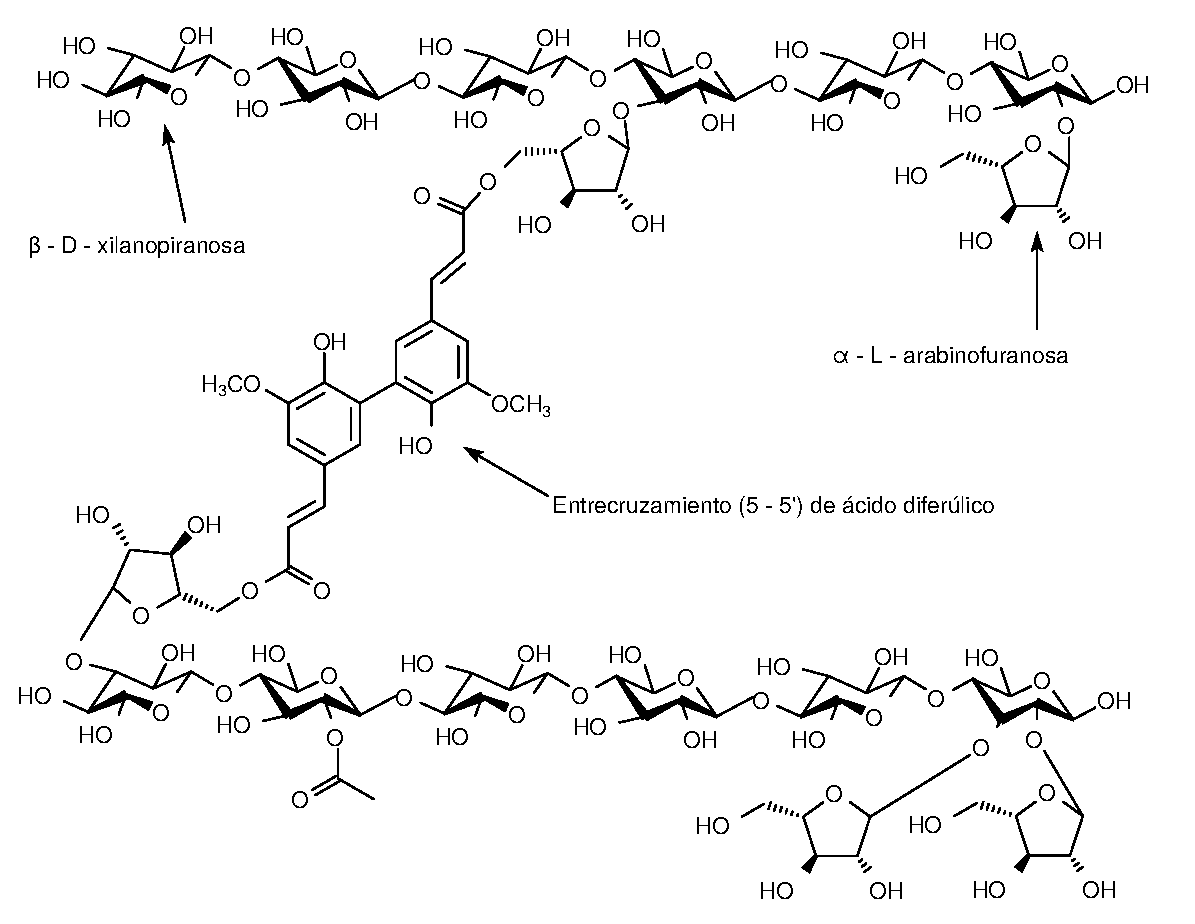
\includegraphics[width=1\linewidth]{CrossLink.pdf}
    \caption[Estructura química de hidrogeles de AX]%
    {Estructura química de hidrogeles de AX (Obtenida de \citet{andrewartha1979solution}). Oratio iriure rationibus ne his, ad est corrumpit splendide. Eum hinc argumentum te, no sit percipit adversarium, ne qui feugiat persecuti.}
    \label{fig:GelificacionAX}
\end{figure}


% --------------------------------------------------
\subsection{Eum hinc argumentum te}
% --------------------------------------------------
Estas sólo son unas pruebas de acrónimos: \ac{AX}, \acp{AX} ocurre, por defecto añade una s al final. Con \acf{AX} hacemos que aparezca el texto completo del acrónimo, con el comando \acs{AX} hacemos que aparezca la versión córta del acrónimo \footnote{Este texto es para ejemplificar.}. Primero hablaré del \gloss{CoefHuggins}. Después, haré una prueba para utilizar la \gloss{EqHuggins}. Eum hinc argumentum\index{argentum} te, no sit percipit\index{percipite} adversarium\index{adversarium}, ne qui feugiat persecuti\index{persecuti}. Odio omnes scripserit\index{scripserit} ad est, ut vidit lorem maiestatis his, putent mandamus gloriatur ne pro. Oratio\index{oratio} iriure rationibus\index{splendide!rationibus} ne his\index{splendide!Bullet Points}, ad est corrumpit splendide\index{splendide!Bullet Points}.


\begin{table}[htb]
\caption{Tabla demostrativa y notas al pie}
\begin{center}
%\begin{tabular}{ c c c c c }
% ----------------------------------------------------------
\begin{tabularx}{1\textwidth}{ l c c c c }
\toprule
\parnoteclear % tabularx will otherwise add each note thrice
\textbf{Fuente} \parnote{Los datos fueron expresados en g/100 gbs y realizados los ensayos por triplicado} & \textbf{Valor 001} & \textbf{Valor 002} & \textbf{Valor 003} & \textbf{Referencia} \\ 
\midrule
\midrule
nejayote & 5.6 & 4.7 & 6.5 & \citet{arambula2001physicochemical} \\ 
percarpio & 4.5 & 5.5 & 2.3 & \citet{azadi2013liquid} \\ 
harina & 7.8 & 3.9 & 7.4 & \citet{barron2008ftir} \\ 
\bottomrule
\end{tabularx}
% ----------------------------------------------------------
%\end{tabular}
\end{center}
\label{tab:Demo001}
\parnotes
\end{table}

